
\subsection{The Large Hadron Collider}

The Large Hadron Collider (LHC), located at CERN near Geneva, is the largest and highest-energy particle accelerator in the world.  It consists of two counter-rotating particle beam line in a tunnel 26.7 km in circumference, located between 45 m and 170 m underground~\cite{Evans:2008zzb}.  During standard operation, the LHC collides beams of protons accelerated and focused using a series of superconducting magnets, cooled to below 2 K using supercritical helium.  Particle beams are brought together for collisions at in experimental detectors at four points in the accelerator ring:  the ATLAS, CMS, ALICE, and LHCb detectors.  In addition to the proton-proton (pp) data collected at center-of-mass energies $\sqrt{\rm S_{NN}} = 7$ TeV, 8 TeV, and 13 TeV, the LHC has also been operated for heavy ion physics by colliding with fully-stripped lead nuclei ($\rm ^{182}Pb^{82+}$) in lead-lead (PbPb) and proton-lead (pPb) collisions.  Heavy ion runs at the LHC have included PbPb data and pp ``reference'' runs at $\sqrt{\rm S_{NN}} = 2.76$ TeV (2011 and 2013, respectively) and 5.02 TeV (2015) and pPb data at $\sqrt{\rm S_{NN}} = 5.02$ TeV (2013 and 2016) and 8.16 TeV (2016).  This analysis relies on PbPb data at 2.76 TeV and 5.02 TeV, and corresponding pp reference data at the same center-of-mass energies. 

In peak proton-proton operation, the LHC collides 2,808 bunches each containing approximately $10^{11}$ protons with a minimum bunch spacing of 25 ns, for a maximum luminosity of $10^{34}\rm cm^{-2}s^{-1}$ delivered to the high-luminosity detectors (ATLAS and CMS).  The lead-lead performance target of $10^{27}\rm cm^{-2}s^{-1}$ delivered via 592 bunches of $10^{7}$ lead ions was slightly exceeded during the 2015 PbPb run.  At this high-intensity frontier, it is common during nominal pp data collection and possible in PbPb data collection that multiple distinct proton-proton collisions may occur within a recorded event in a phenomenon known as ``pile-up.''  However, pile-up is relatively rare in PbPb collisions due to the lower luminosities, and in the present analysis only one primary vertex will be considered (with products of any other possible interactions removed via background subtraction procedures). 

\subsection{The CMS detector}

The CMS detector is named for the Compact Muon Solenoid at its heart:  a superconducting magnet with magnetic field of 3.8 T, length of 13 m, diameter of 6 m, and weight 14,000 tons.  Inside of this solenoid, the detector includes silicon pixel and strip detectors for particle tracking (see Sec.~\ref{sec:trackers} for a detailed explanation), and electromagnetic and hadronic calorimeters (see Sec.~\ref{sec:calorimeters}).  Calorimeters within the solenoid volume are complemented by additional calorimetry outside of the solenoid that provides coverage in the very forward direction close to the beam line, including the hadronic forward (HF) calorimeter in the region $3.0 < |\eta| < 5.2$ used in this analysis for centrality determination, and the Zero Degree and CASTOR calorimeters in the even more forward region.  The CMS detector also includes an extensive muon system outside of the solenoid volume, consisting of aluminum drift tubes in the barel region, cathode strip chambers in the forward region, and a complementary system of resistive plate chambers (not discussed in detail here as muons are not of primary relevance to this analysis).  Full details about the CMS detector may be found in Ref.~\cite{Chatrchyan:2008zzk}, and a perspective drawing of the CMS detector from this report is shown in Fig.~\ref{fig:detector}.

In the CMS detector, the +z axis is defined to be horizontal, pointing to the West along the beam line direction.  The x axis is horizontal, pointing to the South toward the center of the LHC.  The +y axis is vertical, pointing upward.  The azimuthal angle $\phi = \rm tan^{-1}(\frac{y}{x})$ is defined in the x-y plane such that $\phi = 0$ is the +x axis.  Pseudorapidity $\eta = \rm -ln(tan(\frac{\theta}{2})$ is defined to have the same sign as the +z axis.  Pseudorapidity coverage in the CMS detector ranges from $\eta = 0$ at the y-axis, to $|\eta| > 8.3$ in Zero Degree Calorimeter approaching the +/-z axis.

\begin{figure}[hbtp]
\begin{center}
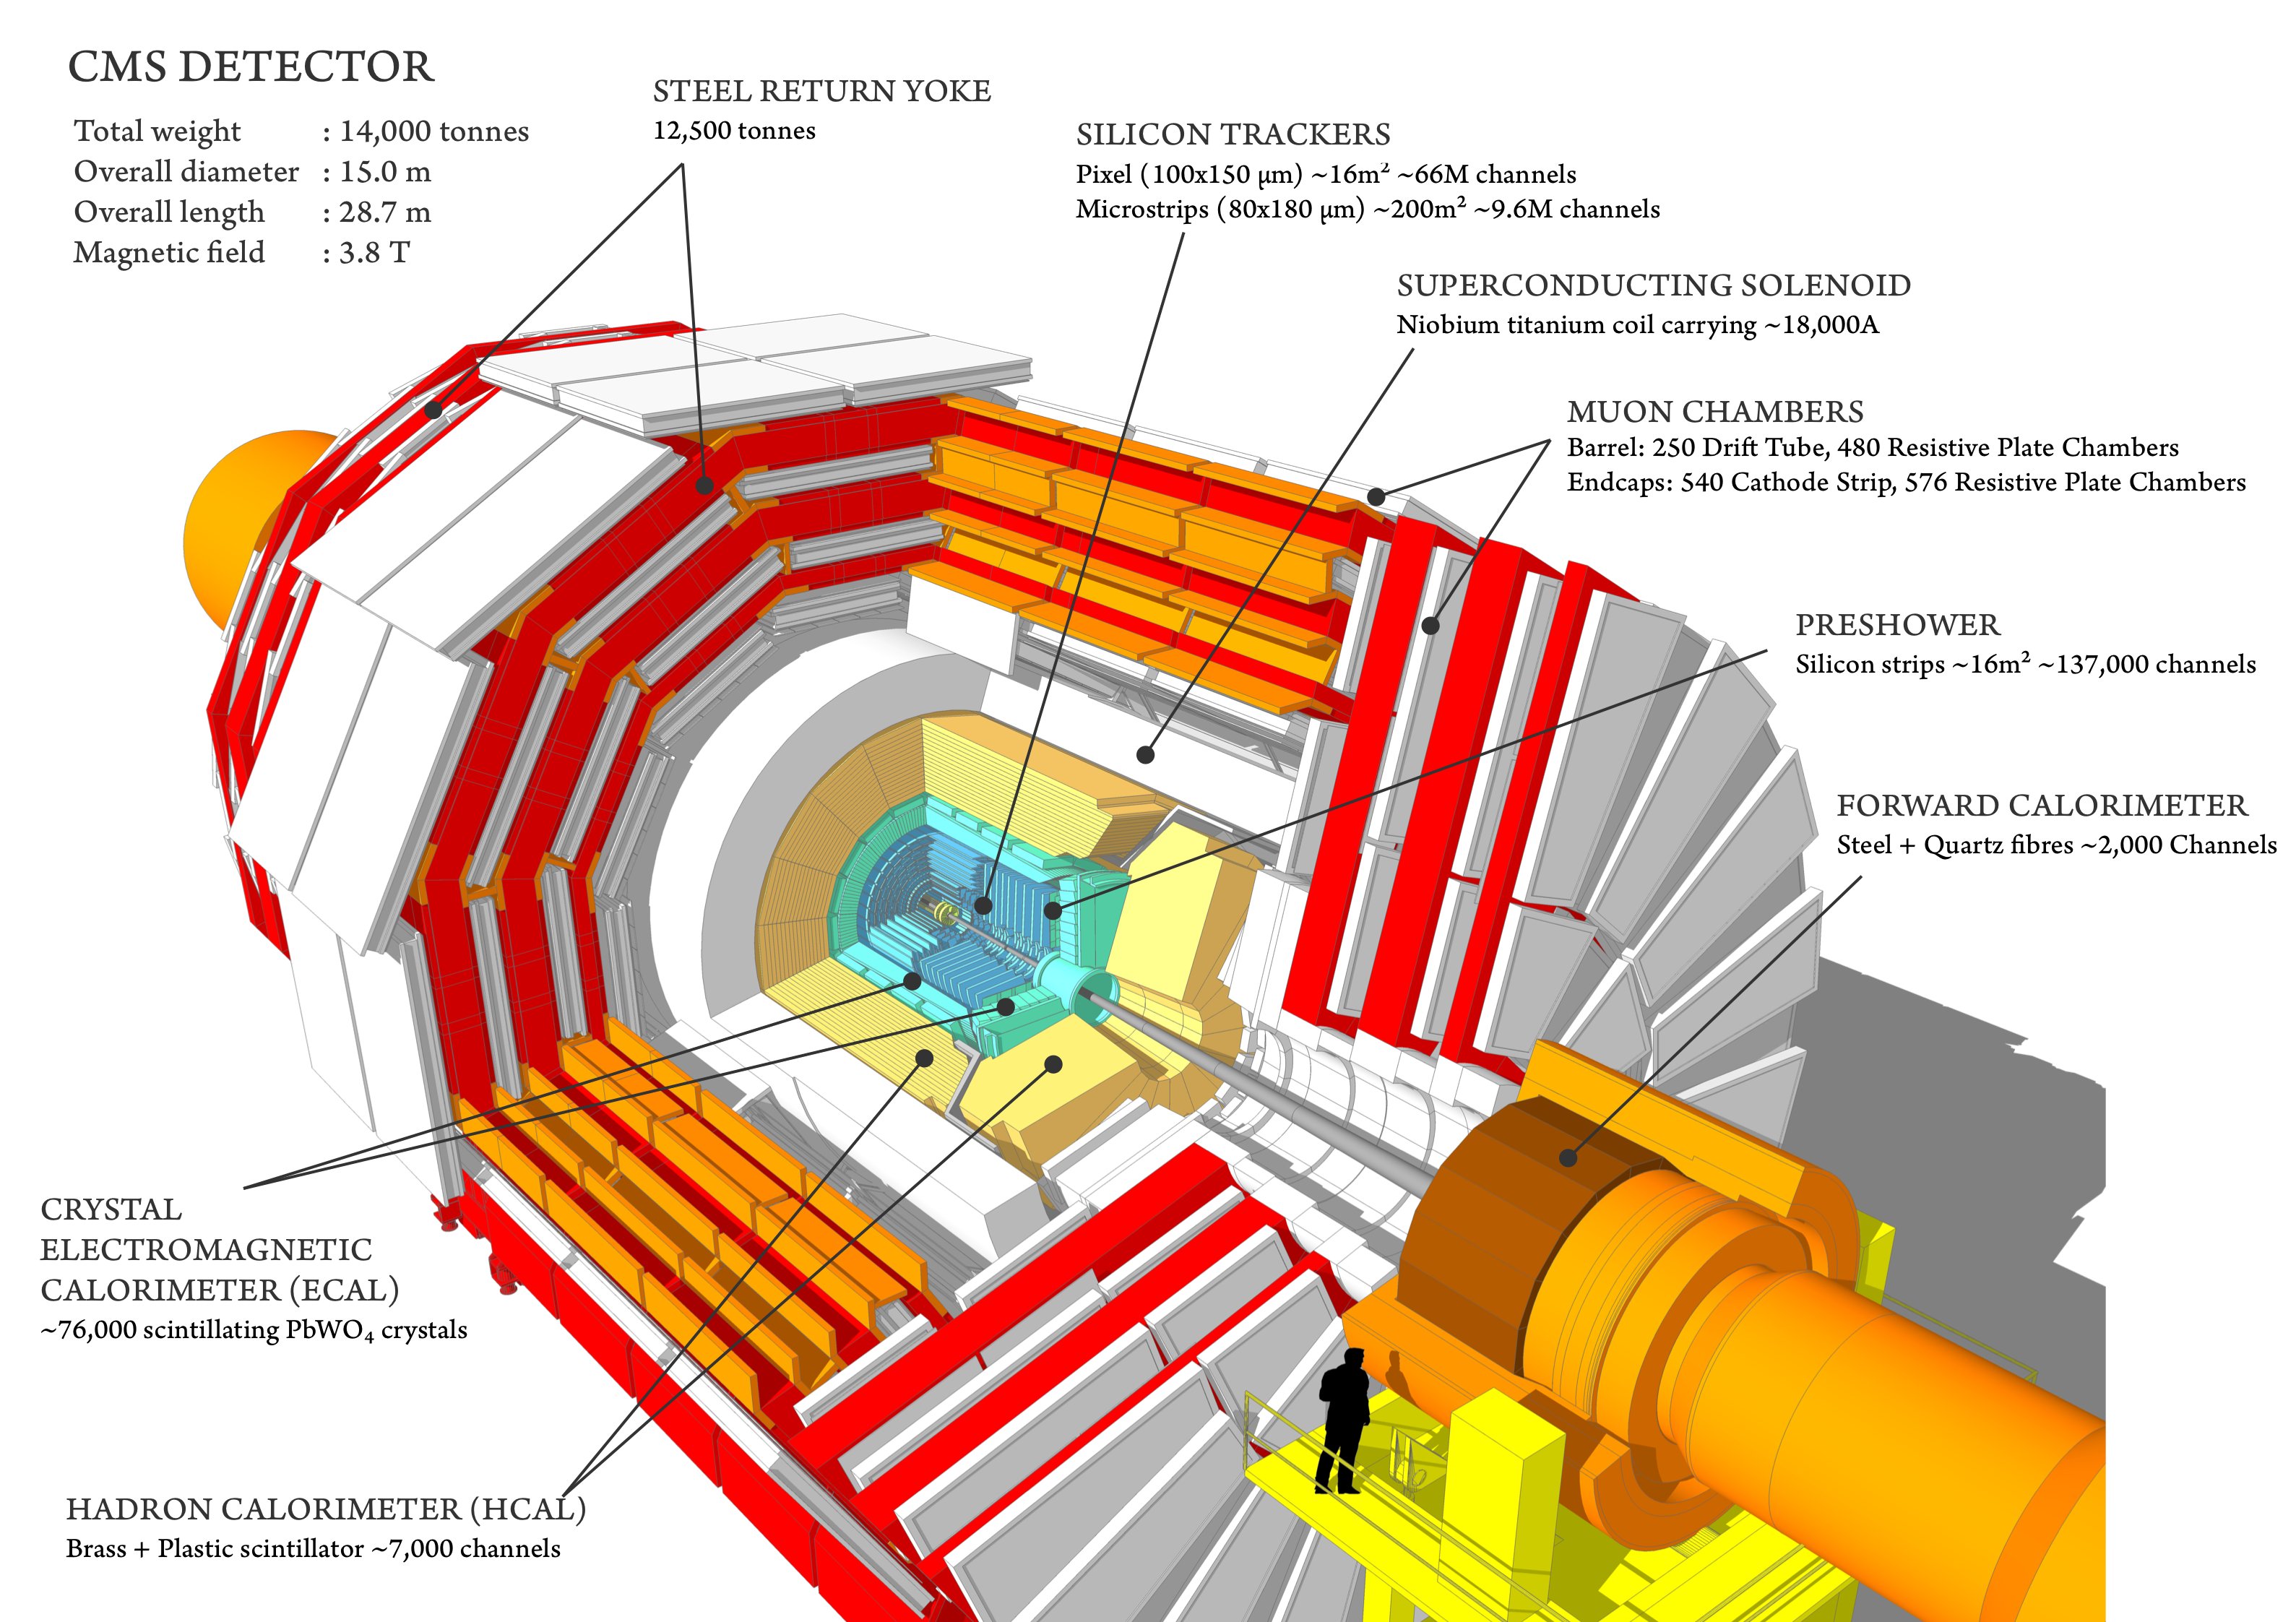
\includegraphics[width=0.9\textwidth]{figures/Detector/Detector.png}
\caption[CMS detector perspective drawing]{Perspective rendering of the CMS detector, showing component sub-detectors with a human included for scale perspective~\cite{SketchUp}.}
\label{fig:detector}
\end{center}
\end{figure}

\subsection{Trackers in the CMS detector}
\label{sec:trackers}

The CMS tracking system consists of a small silicon pixel detector for precise measurement near the interaction point (with three layers with radii 4.4 cm to 10.2 cm), surrounded by a large silicon strip detector with layers to a radius of 110 cm.  In both detectors, a cylindrical tracker ``barrel'' is complemented by ``endcap'' disks that together provide full azimuthal coverage and pseudorapidity coverage in the range $|\eta| < 2.5$.  The pixel detector consists of 66 million pixels in 1440 modules.  It provides three-dimensional measurements of ``hits,'' or interactions of particles with tracker materials, with a transverse resolution $10 \mu$m and longitudinal resolution $20 - 40 \mu$m (and a third coordinate provided by the pixel plane).  The silicon strip detector consists of 9.3 million strips in 15,148 modules, organized in four components:  Tracker Inner Barrel (TIB) and Disks (TID), Tracker Outer Barrel (TOB, covering the region $r > 55 \rm$ cm), and Tracker End Caps (TEC, covering the region $124 < |z| < 282$ cm).  Figure~\ref{fig:tracker} shows a diagram of the pixel and strip detectors, which have total length 5.8 m and diameter 2.5 m~\cite{Chatrchyan:2014fea}.  Track reconstruction and tracking efficiency will be discussed in detail in Sec.~\ref{sec:Tracks}.


\begin{figure}[hbtp]
\begin{center}
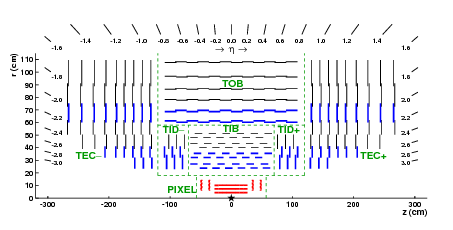
\includegraphics[width=0.7\textwidth]{figures/Detector/figs_2011_cmsTracker_TrackerLayoutNew.png}
\caption[Diagram of CMS trackers]{Diagram of CMS pixel and silicon strip detectors in the $r-z$ plane~\cite{Chatrchyan:2014fea}.}
\label{fig:tracker}
\end{center}
\end{figure}



\subsection{Calorimeters in the CMS detector}
\label{sec:calorimeters}

This analysis relies on electromagnetic and hadronic calorimeters for the energy measurements used as inputs for the reconstruction of high-$p_{\rm T}$ jets.  The ECAL, which measures the energy of charged particles, consists of 75\,848 lead tungstate ($\rm PbWO_{4}$) crystal scintillators, organized in $5 \time 5$ arrays, covering $|\eta| < 1.48 $ in a barrel region and $1.48 < |\eta| < 3.0$ in the endcap region.  Light from the scintillators is captured with avalanche photodiodes in the barrel region, and vacuum phototriodes in the endcap region.  A preshower detector system in front of the ECAL is used to assist in the identification of neutral pions and electrons~\cite{Chatrchyan:2008zzk}.  ECAL energy resolution ranges from about 1-2.5\% (depending $|\eta|$ and photon conversion) in the barrel region, and from 2.5-4\% in the endcap region.~\cite{CMS:EGM-14-001}. 

Hadrons pass through the ECAL and are stopped by the HCAL, a hermetic detector which records their energy using a system of scintellator tiles embedded with wavelength-shifting  fibers.  The HCAL has three regions, as shown in Fig.~\ref{fig:HCAL}:  barrel (HB), endcap (HE), and an outer region (HO) outside of the solenoid, necessitated by the fact that the HB is volume-limited by the solenoid diameter.  In the barrel region $|\eta| < 1.74$, the HCAL cells have widths of 0.087 in pseudorapidity and 0.087 in $\phi$, while for $|\eta| > 1.74$ the coverage of the towers increases progressively to a maximum of 0.174 in $\Delta \eta$ and $\Delta \phi$.  HCAL towers are mapped onto ECAL towers within the barrel region, and their summed energies are used to determine the location, energy, and axis of jets, as described below in Sec.~\ref{sec:Jets}.  The HCAL is complimented in the forward region by the HF calorimeters, which each consist quartz fibers in the $\pm z$ directions organized in 432 readout towers in the region $3.0 < |\eta| < 5.2$~\cite{Chatrchyan:2008zzk}.  In this analysis, only jets from the barrel region of the calorimeters wil be included, while the HF detector is used for the determination of PbPb event centrality as described in Sec.~\ref{sec:centrality}. 

\begin{figure}[h!]
\begin{center}
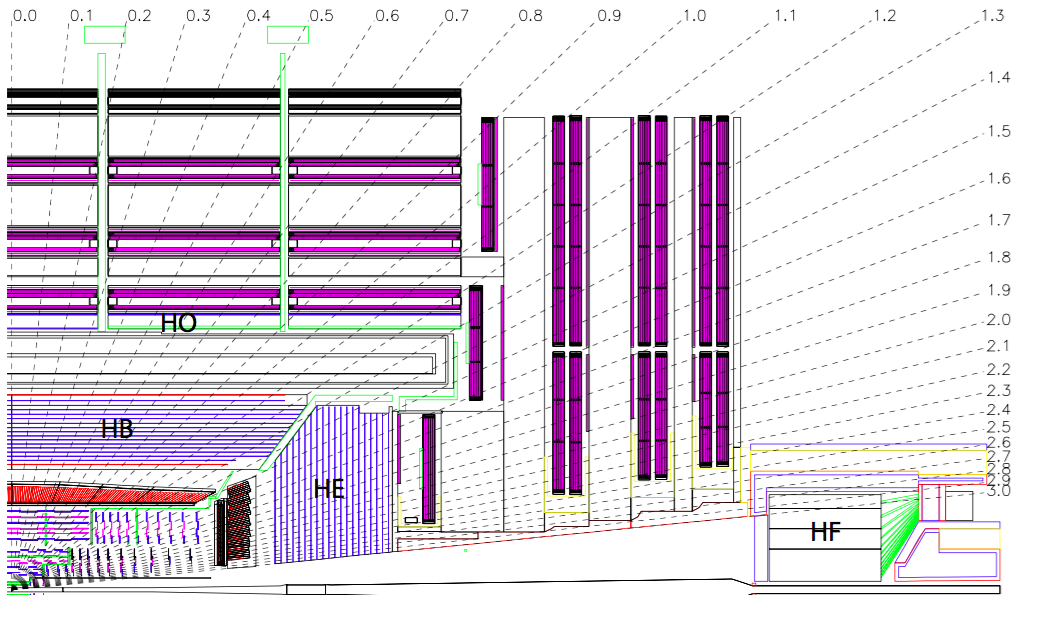
\includegraphics[width=0.6\textwidth]{figures/Detector/HCAL_Diagram.png}
\caption[Diagram of the HCAL]{Diagram of the HCAL~\cite{Chatrchyan:2008zzk}.}
\label{fig:HCAL}
\end{center}
\end{figure}

\subsection{The CMS trigger system}
\label{sec:HLT}

The collision rate at in the LHC is so high that it is impossible to store and process every event that occurs in the CMS detector.  A two-level online trigger system is therefore used to select events of interest.  Furthermore, data selected with loose trigger requirements (for example ``zero bias'' data with no selection criteria and ``minimum bias'' criteria consisting of minimal requirements to demonstrate the presence of a collision event) may also need to be further ``prescaled'' to limit the rate of recorded events by a specified factor.  The trigger system consists of a first (L1) trigger consisting of progammable electronics that use information from the calorimeter and muon systems of the detector to select events to record.  The L1 trigger opperates with an interval of approximately $4 \mu$ s, with a maximum rate of 100 kHz.  The next trigger level, the High Level Trigger (HLT), consists of a processor farm that allows for more sophisticated event selection based on the reconstruction of physics objects.  Reconstruction is performed in a series of steps, or a ``HLT path,'' chosen to apply selection in order of increasing reconstruction complexity, so as to minimize processing time~\cite{Khachatryan:2016bia}.  This analysis will rely primarily on two kinds of triggers:  minimum bias data, and jet-triggered data samples selected by requiring the presence of an online reconstructed jet with $p_{\rm T} > 80 $ GeV ($p_{\rm T} > 100 $ GeV for 5.02 TeV PbPb data).  No prescale is applied for the jet-triggered data samples used in this analysis.  





